\documentclass[10pt]{article}
\usepackage[margin=0.58in]{geometry}
\usepackage{amsmath,amssymb,mathtools,xcolor,tikz,tikz-cd,fancyvrb,fontspec,multicol,booktabs}
\usetikzlibrary{arrows.meta,automata,backgrounds,calc,cd,decorations.pathmorphing,decorations.pathreplacing,
  decorations.markings,fit,intersections,matrix,patterns,positioning,
  quotes,shapes.geometric,shapes.misc,trees}
\pagestyle{empty}
\setlength{\parindent}{0pt}
\setlength{\parskip}{2pt}
\definecolor{ink}{RGB}{28,35,49}
\definecolor{blue}{RGB}{35,91,160}
\definecolor{red}{RGB}{155,47,47}
\definecolor{green}{RGB}{28,125,91}
\definecolor{gold}{RGB}{184,126,15}
\definecolor{pale}{RGB}{240,244,249}
\color{ink}
\newfontfamily\leanfont{DejaVu Sans}
\newenvironment{lean}{\Verbatim[fontsize=\scriptsize,frame=single,framesep=1.5mm,rulecolor=\color{blue},formatcom=\leanfont]}{\endVerbatim}
\newcommand{\injdim}{\operatorname{idim}}
\newcommand{\ModCat}{\mathbf{Mod}}
\newcommand{\rang}{\operatorname{range}}
\newcommand{\inj}{\mathsf{Inj}}
\newcommand{\smalltag}[1]{\tikz[baseline=(X.base)]\node[fill=pale,rounded corners=2pt,inner sep=2pt] (X) {\scriptsize #1};}
\begin{document}

\begin{center}
{\LARGE\bfseries Injective dimension survives change of coordinates}\\[-1mm]
{\large A visual mathematical reading and PR review of the Lean diff}
\end{center}

\begin{center}
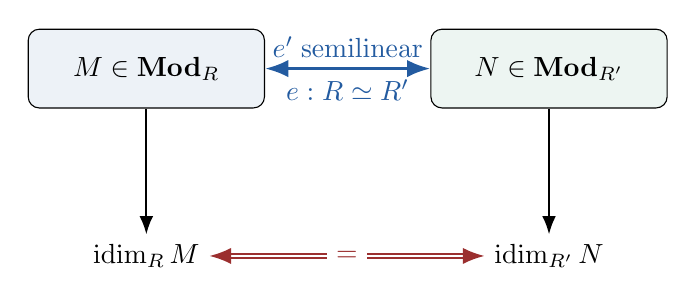
\begin{tikzpicture}[>=Latex,node distance=14mm and 21mm]
\node[draw,rounded corners,fill=blue!8,minimum width=30mm,minimum height=10mm] (M) {$M\in\ModCat_R$};
\node[draw,rounded corners,fill=green!8,right=of M,minimum width=30mm,minimum height=10mm] (N) {$N\in\ModCat_{R'}$};
\draw[<->,very thick,blue] (M) -- node[above] {$e'\;\text{semilinear}$} node[below] {$e:R\simeq R'$} (N);
\node[below=16mm of M] (dM) {$\injdim_R M$};
\node[below=16mm of N] (dN) {$\injdim_{R'}N$};
\draw[->,thick] (M)--(dM); \draw[->,thick] (N)--(dN);
\draw[<->,double,red,thick] (dM)--node[fill=white] {$=$}(dN);
\end{tikzpicture}
\end{center}

\[
\boxed{\quad M\simeq_{e,\mathrm{semi}}N\quad\Longrightarrow\quad
\injdim_R(M)=\injdim_{R'}(N).\quad}
\]

\begin{lean}
lemma injectiveDimension_eq_of_semiLinearEquiv [Small.{v'} R']
    {M : ModuleCat.{v} R} {N : ModuleCat.{v'} R'}
    (e' : M ≃ₛₗ[RingHomClass.toRingHom e] N) :
    injectiveDimension M = injectiveDimension N := by
  ...
\end{lean}

\vfill
\begin{center}\small
\textcolor{green}{\bfseries Verdict:} mathematically structural and sound in shape.\quad
\textcolor{red}{\bfseries Before merge:} title fix + dead-line deletion.\quad
\textcolor{blue}{\bfseries Follow-up:} exact-equivalence transport API.
\end{center}
\newpage

\section*{1. The invariant: shortest injective resolution}

\begin{center}
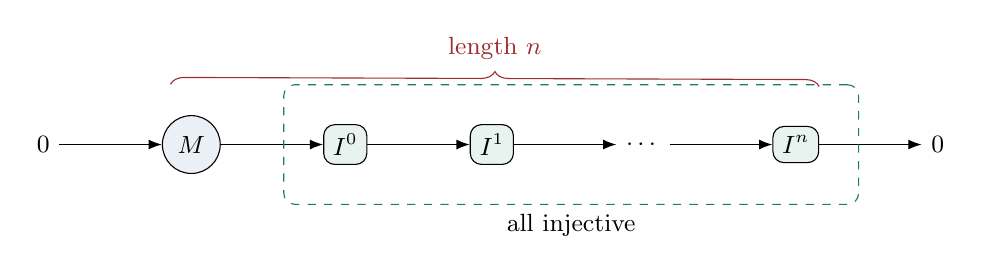
\begin{tikzpicture}[>=Latex,node distance=12mm and 13mm,every node/.style={font=\small}]
\node (z) {$0$};
\node[right=of z,draw,circle,fill=blue!9] (M) {$M$};
\node[right=of M,draw,rounded corners,fill=green!10] (I0) {$I^0$};
\node[right=of I0,draw,rounded corners,fill=green!10] (I1) {$I^1$};
\node[right=of I1] (dots) {$\cdots$};
\node[right=of dots,draw,rounded corners,fill=green!10] (In) {$I^n$};
\node[right=of In] (zz) {$0$};
\foreach \a/\b in {z/M,M/I0,I0/I1,I1/dots,dots/In,In/zz} \draw[->] (\a)--(\b);
\node[fit=(I0)(I1)(In),draw=green,dashed,rounded corners,inner sep=5mm,label=below:{all injective}] {};
\draw[decorate,decoration={brace,amplitude=5pt},red] ($(M.north west)+(0,5mm)$)--($(In.north east)+(0,5mm)$)
 node[midway,above=6pt] {$\text{length }n$};
\end{tikzpicture}
\end{center}

\[
\injdim(M)\le n
\quad\Longleftrightarrow\quad
\text{$M$ admits an injective resolution of length at most $n$}.
\]

The code uses the dimension-shifting recurrence rather than manipulating a whole resolution:
\[
0\longrightarrow M\xrightarrow{f}I\longrightarrow C\longrightarrow0,
\qquad I\ \text{injective},
\qquad
\boxed{\injdim(M)\le n+1\iff\injdim(C)\le n.}
\]

\begin{lean}
(exactS.hasInjectiveDimensionLT_X₃_iff n inferInstance)
\end{lean}

\begin{center}
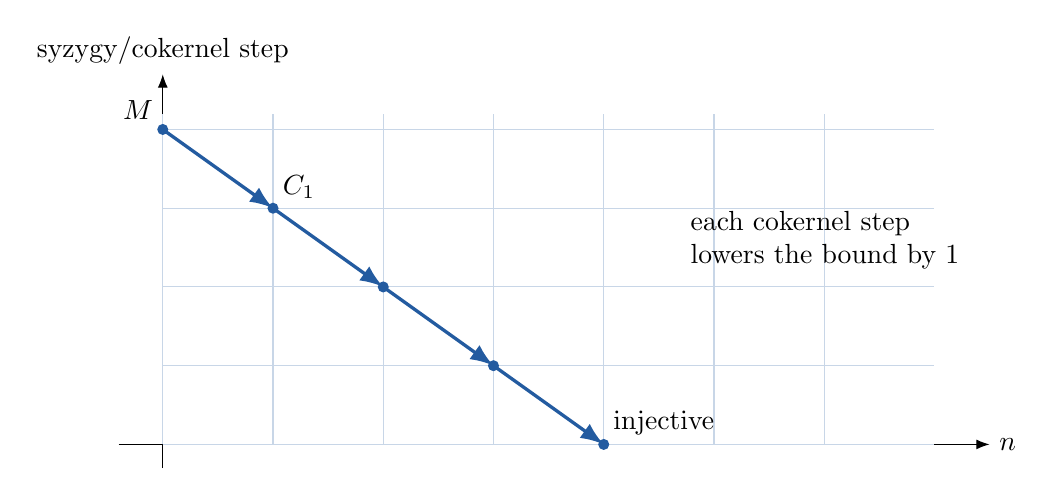
\begin{tikzpicture}[>=Latex,x=14mm,y=10mm]
\draw[->] (-.4,0)--(7.5,0) node[right] {$n$};
\draw[->] (0,-.3)--(0,4.7) node[above] {syzygy/cokernel step};
\foreach \x in {0,...,6} \draw[blue!25] (\x,0)--(\x,4.2);
\foreach \y in {0,...,4} \draw[blue!25] (0,\y)--(7,\y);
\foreach \k in {0,...,4} {
  \fill[blue] (\k,4-\k) circle (2pt);
  \ifnum\k<4 \draw[very thick,blue,-{Latex}] (\k,4-\k)--(\k+1,3-\k);\fi
}
\node[above left] at (0,4) {$M$};
\node[above right] at (1,3) {$C_1$};
\node[above right] at (4,0) {injective};
\node[align=left,anchor=west] at (4.7,2.6) {each cokernel step\\lowers the bound by $1$};
\end{tikzpicture}
\end{center}

\section*{2. Base case: Baer transport}

At $n=0$, dimension zero means injective.  A linear equivalence preserves the ideal-extension
criterion (Baer's criterion):
\[
\injdim(M)\le0\iff M\text{ injective}
\iff N\text{ injective}\iff\injdim(N)\le0.
\]

\begin{lean}
simp [HasInjectiveDimensionLE, ← injective_iff_hasInjectiveDimensionLT_one,
  ← Module.injective_iff_injective_object R M,
  ← Module.injective_iff_injective_object R N,
  ← Module.Baer.iff_injective, Module.Baer.congr e]
\end{lean}

\newpage
\section*{3. Inductive engine: two short exact rows}

\begin{center}
\begin{tikzcd}[column sep=1.65em,row sep=3.0em,cells={nodes={font=\small}}]
0 \arrow[r] & M \arrow[r,"f"] \arrow[d,"e'"',"\sim"]
& I \arrow[r,"q"] \arrow[d,"e_I"',"\sim"]
& C=I/\rang(f) \arrow[r] \arrow[d,"e_C"',"\sim"] & 0 \\
0 \arrow[r] & N \arrow[r,"f'"]
& I' \arrow[r,"q'"]
& C'=I'/\rang(f') \arrow[r] & 0
\end{tikzcd}
\end{center}

\begin{center}
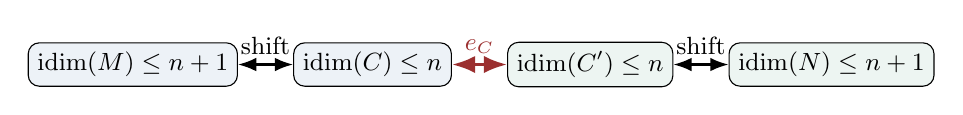
\begin{tikzpicture}[node distance=7mm,>=Latex,every node/.style={font=\small}]
\node[draw,rounded corners,fill=blue!8] (a) {$\injdim(M)\le n+1$};
\node[draw,rounded corners,fill=blue!8,right=of a] (b) {$\injdim(C)\le n$};
\node[draw,rounded corners,fill=green!8,right=of b] (c) {$\injdim(C')\le n$};
\node[draw,rounded corners,fill=green!8,right=of c] (d) {$\injdim(N)\le n+1$};
\draw[<->,thick] (a)--node[above]{shift}(b);
\draw[<->,very thick,red] (b)--node[above]{$e_C$}(c);
\draw[<->,thick] (c)--node[above]{shift}(d);
\end{tikzpicture}
\end{center}

This four-arrow chain is the proof.

\begin{lean}
exact (exactS.hasInjectiveDimensionLT_X₃_iff n inferInstance).symm.trans
  ((ih eCoker).trans
    (exactS'.hasInjectiveDimensionLT_X₃_iff n inferInstance))
\end{lean}

\subsection*{Canonical short exact sequence}

\begin{lean}
let S : ShortComplex (ModuleCat.{v} R) :=
  ModuleCat.shortComplexOfCompEqZero _ _
    f.hom.exact_map_mkQ_range.linearMap_comp_eq_zero
have exactS := ModuleCat.shortComplex_shortExact S
  f.hom.exact_map_mkQ_range injf (Submodule.mkQ_surjective _)
\end{lean}

\begin{center}
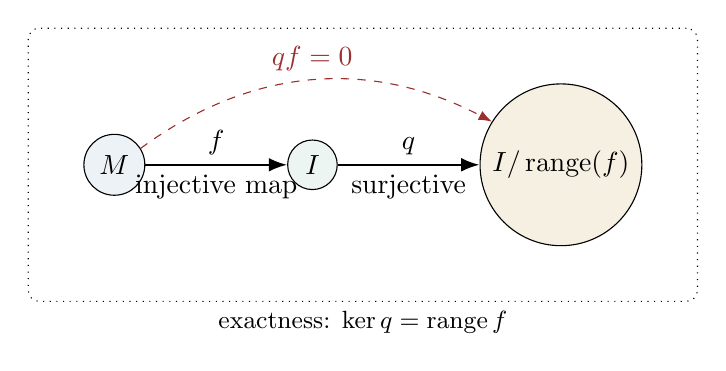
\begin{tikzpicture}[>=Latex,node distance=18mm]
\node[draw,circle,fill=blue!8] (M) {$M$};
\node[draw,circle,fill=green!8,right=of M] (I) {$I$};
\node[draw,circle,fill=gold!12,right=of I] (Q) {$I/\rang(f)$};
\draw[->,thick] (M)--node[above] {$f$} node[below] {injective map} (I);
\draw[->,thick] (I)--node[above] {$q$} node[below] {surjective} (Q);
\draw[->,bend left=32,dashed,red] (M) to node[above] {$qf=0$} (Q);
\node[fit=(M)(I)(Q),draw,dotted,rounded corners,inner sep=7mm,label=below:{\small exactness: $\ker q=\rang f$}] {};
\end{tikzpicture}
\end{center}

\smalltag{Improvement} Package this repeated construction as a canonical short-exact-sequence helper.

\section*{4. The quotient equivalence, geometrically}

\begin{center}
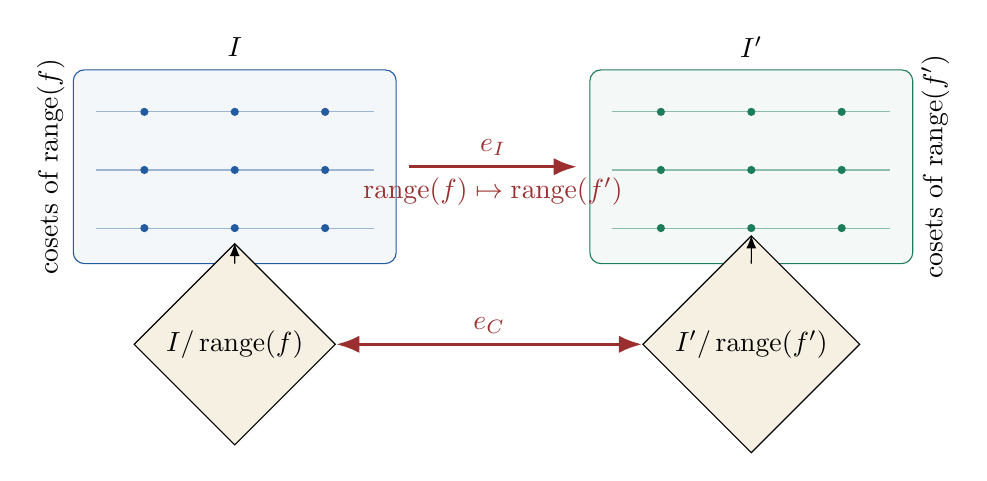
\begin{tikzpicture}[>=Latex,scale=.82]
\draw[fill=blue!5,draw=blue,rounded corners] (0,0) rectangle (5,3);
\foreach \y in {.55,1.45,2.35} {
  \draw[blue!45] (.35,\y)--(4.65,\y);
  \fill[blue] (1.1,\y) circle (1.8pt); \fill[blue] (2.5,\y) circle (1.8pt); \fill[blue] (3.9,\y) circle (1.8pt);
}
\node at (2.5,3.35) {$I$}; \node[rotate=90] at (-.35,1.5) {cosets of $\rang(f)$};
\draw[fill=green!5,draw=green,rounded corners] (8,0) rectangle (13,3);
\foreach \y in {.55,1.45,2.35} {
  \draw[green!50] (8.35,\y)--(12.65,\y);
  \fill[green] (9.1,\y) circle (1.8pt); \fill[green] (10.5,\y) circle (1.8pt); \fill[green] (11.9,\y) circle (1.8pt);
}
\node at (10.5,3.35) {$I'$}; \node[rotate=90] at (13.35,1.5) {cosets of $\rang(f')$};
\draw[->,very thick,red] (5.2,1.5)--node[above] {$e_I$} node[below] {$\rang(f)\mapsto\rang(f')$} (7.8,1.5);
\node[draw,diamond,fill=gold!12] (q1) at (2.5,-1.25) {$I/\rang(f)$};
\node[draw,diamond,fill=gold!12] (q2) at (10.5,-1.25) {$I'/\rang(f')$};
\draw[->] (2.5,0)--(q1); \draw[->] (10.5,0)--(q2);
\draw[<->,very thick,red] (q1)--node[above] {$e_C$} (q2);
\end{tikzpicture}
\end{center}

For classes $[i]$, the induced map is
\[
e_C([i])=[e_I(i)],
\qquad e_C^{-1}([i'])=[e_I^{-1}(i')].
\]
Well-definedness is exactly
\(
ang(f)\xmapsto{e_I}\rang(f')\).

\begin{lean}
have eqmap : f'.hom.range.map eI.symm.toLinearMap = f.range := by
  simp [f, LinearMap.range_comp]
let eCoker : ModuleCat.of R (I / f.range) ≃ₛₗ[RingHomClass.toRingHom e]
    ModuleCat.of R' (I' / f'.hom.range) := {
  __ := Submodule.mapQ _ _ eI.toLinearMap ...
  invFun := Submodule.mapQ _ _ eI.symm.toLinearMap ...
  left_inv x := Submodule.Quotient.induction_on _ x (by simp)
  right_inv x := Submodule.Quotient.induction_on _ x (by simp) }
\end{lean}

\smalltag{Improvement} Add reusable API: semilinear equivalence + mapped-submodule equality
$\Rightarrow$ quotient semilinear equivalence.

\newpage
\section*{5. Change of scalars is a categorical equivalence}

A ring equivalence changes scalar notation, not module geometry:
\[
e:R\simeq R',\qquad e':M\simeq_{e,\mathrm{semi}}N,
\qquad e'(rm)=e(r)e'(m).
\]

\begin{center}
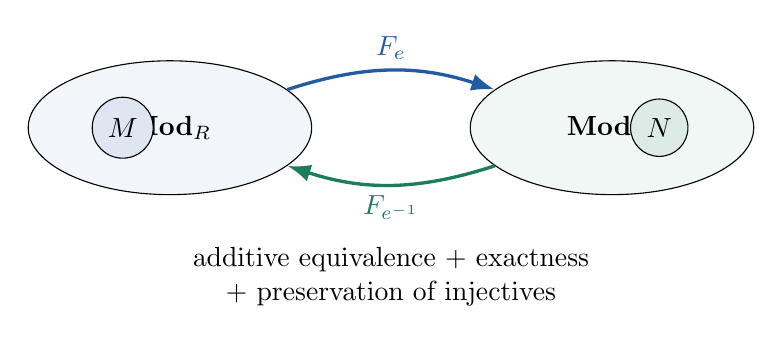
\begin{tikzpicture}[>=Latex,node distance=20mm]
\node[draw,ellipse,minimum width=36mm,minimum height=17mm,fill=blue!6] (R) {$\ModCat_R$};
\node[draw,ellipse,minimum width=36mm,minimum height=17mm,fill=green!6,right=of R] (Rp) {$\ModCat_{R'}$};
\draw[->,very thick,blue,bend left=18] (R) to node[above] {$F_e$} (Rp);
\draw[->,very thick,green,bend left=18] (Rp) to node[below] {$F_{e^{-1}}$} (R);
\node[draw,circle,fill=blue!15] at ($(R.center)+(-.6,0)$) {$M$};
\node[draw,circle,fill=green!15] at ($(Rp.center)+(.6,0)$) {$N$};
\node[below=14mm of $(R)!0.5!(Rp)$,align=center] {additive equivalence + exactness\\$+$ preservation of injectives};
\end{tikzpicture}
\end{center}

The implementation rebuilds the transported middle term:

\begin{lean}
let I : ModuleCat.{v} R :=
  let := Module.compHom I' e.toRingHom
  ModuleCat.of R I'
let eI : I ≃ₛₗ[RingHomClass.toRingHom e] I' := {
  __ := AddEquiv.refl I
  map_smul' r i := rfl }
\end{lean}

Injectivity crosses the equivalence:

\begin{lean}
have : Injective (ModuleCat.of R I) := by
  rw [← Module.injective_iff_injective_object]
  exact Module.Injective.of_ringEquiv e.symm eI.symm
\end{lean}

\subsection*{The unusually structural general theorem}

\begin{center}
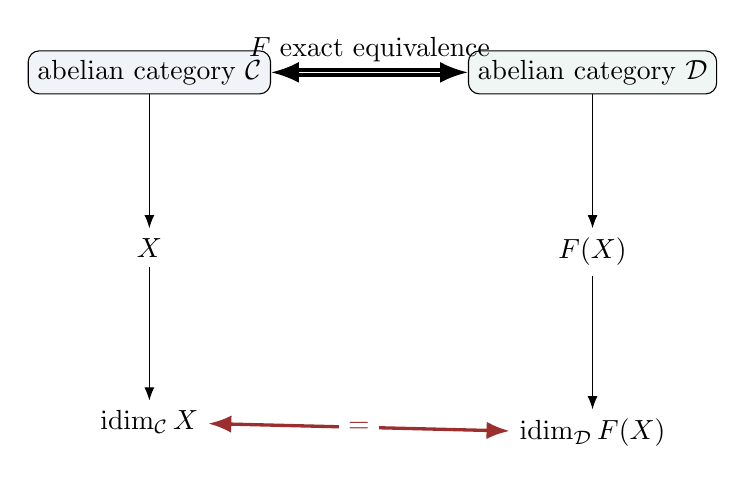
\begin{tikzpicture}[>=Latex,node distance=17mm and 25mm]
\node[draw,rounded corners,fill=blue!7] (C) {abelian category $\mathcal C$};
\node[draw,rounded corners,fill=green!7,right=of C] (D) {abelian category $\mathcal D$};
\draw[<->,double,very thick] (C)--node[above] {$F$ exact equivalence}(D);
\node[below=of C] (X) {$X$}; \node[below=of D] (FX) {$F(X)$};
\draw[->] (C)--(X); \draw[->] (D)--(FX);
\node[below=of X] (ix) {$\injdim_{\mathcal C}X$};
\node[below=of FX] (ifx) {$\injdim_{\mathcal D}F(X)$};
\draw[->] (X)--(ix); \draw[->] (FX)--(ifx);
\draw[<->,very thick,red] (ix)--node[fill=white] {$=$}(ifx);
\end{tikzpicture}
\end{center}

\[
F:\mathcal C\simeq\mathcal D\text{ exact}
\quad\Longrightarrow\quad
\injdim_{\mathcal C}(X)=\injdim_{\mathcal D}(F X).
\]

\smalltag{Design direction} Prove this once in the abelian-category API; derive the module theorem.
It removes manual transport of injectives, ranges, and quotient representatives.

\section*{6. Universe bridge: move both objects to one floor}

\begin{center}
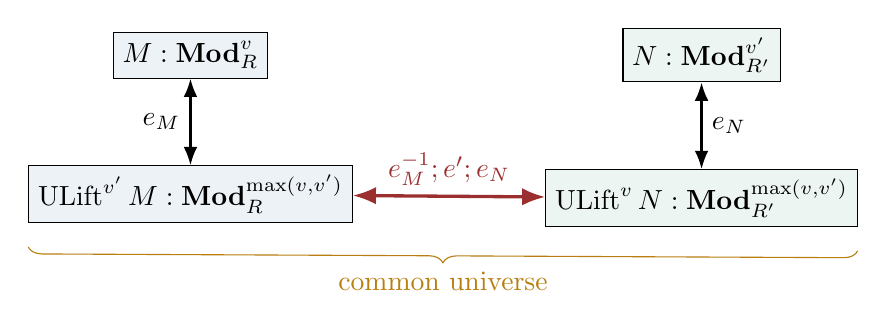
\begin{tikzpicture}[>=Latex,node distance=11mm and 20mm]
\node[draw,fill=blue!8] (M) {$M:\ModCat_R^{v}$};
\node[draw,fill=green!8,right=45mm of M] (N) {$N:\ModCat_{R'}^{v'}$};
\node[draw,fill=blue!8,below=of M] (uM) {$\operatorname{ULift}^{v'}M:\ModCat_R^{\max(v,v')}$};
\node[draw,fill=green!8,below=of N] (uN) {$\operatorname{ULift}^{v}N:\ModCat_{R'}^{\max(v,v')}$};
\draw[<->,thick] (M)--node[left] {$e_M$}(uM);
\draw[<->,thick] (N)--node[right] {$e_N$}(uN);
\draw[<->,very thick,red] (uM)--node[above] {$e_M^{-1};e';e_N$}(uN);
\draw[decorate,decoration={brace,mirror,amplitude=5pt},gold] ($(uM.south west)+(0,-3mm)$)--($(uN.south east)+(0,-3mm)$)
 node[midway,below=5pt] {common universe};
\end{tikzpicture}
\end{center}

\begin{lean}
let eM : M ≃ₗ[R] ModuleCat.of R (ULift.{v'} M) := ULift.moduleEquiv.symm
let eN : N ≃ₗ[R'] ModuleCat.of R' (ULift.{v} N) := ULift.moduleEquiv.symm
rw [hasInjectiveDimensionLE_iff_of_linearEquiv_aux eM,
  hasInjectiveDimensionLE_iff_of_linearEquiv_aux eN]
...
exact hasInjectiveDimensionLE_iff_of_semiLinearEquiv_aux e
  ((eM.symm.trans e').trans eN) n
\end{lean}

\smalltag{Keep} This is explicit, readable, and preferable to opaque coercion tricks.

\newpage
\section*{7. From all bounds to equality in $\mathbb N_\infty$}

The dimension takes values in extended naturals.  Equality is tested by all upper cuts:
\[
a=b\quad\Longleftrightarrow\quad\forall d\in\mathbb N_\infty,\;
(d\le a\Longleftrightarrow d\le b).
\]

\begin{center}
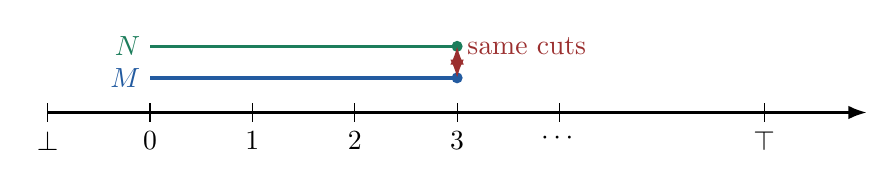
\begin{tikzpicture}[>=Latex,x=13mm,y=8mm]
\draw[->,thick] (0,0)--(8,0);
\foreach \x/\lab in {0/$\bot$,1/$0$,2/$1$,3/$2$,4/$3$,5/$\cdots$,7/$\top$} {
 \draw (\x,.15)--(\x,-.15) node[below] {\lab};
}
\draw[blue,very thick] (1,.55)--(4,.55); \fill[blue] (4,.55) circle (2pt);
\draw[green,very thick] (1,1.05)--(4,1.05); \fill[green] (4,1.05) circle (2pt);
\node[left,blue] at (1,.55) {$M$}; \node[left,green] at (1,1.05) {$N$};
\draw[red,<->,thick] (4,.55)--(4,1.05) node[right] {same cuts};
\end{tikzpicture}
\end{center}

\begin{lean}
refine eq_of_forall_ge_iff (fun N ↦ ?_)
induction N with
| bot => simpa [injectiveDimension_eq_bot_iff,
    ModuleCat.isZero_iff_subsingleton] using e'.subsingleton_congr
| coe n =>
  induction n with
  | top => simp
  | coe n =>
    norm_cast
    simp only [injectiveDimension_le_iff]
    exact hasInjectiveDimensionLE_iff_of_semiLinearEquiv e e' n
\end{lean}

\smalltag{Naming} Rename the cutoff \texttt{N} to \texttt{d}; \texttt{N} already names a module.

\section*{8. Audit map}

\begin{center}
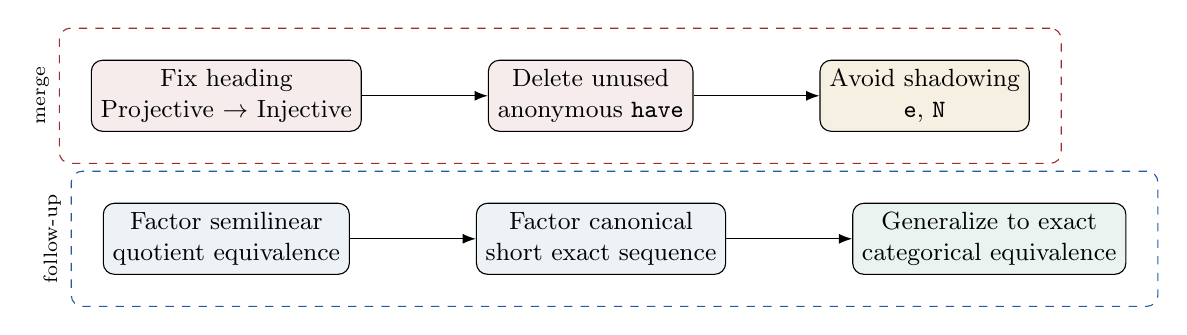
\begin{tikzpicture}[>=Latex,node distance=9mm and 16mm,
  box/.style={draw,rounded corners,align=center,minimum height=8mm,font=\small}]
\node[box,fill=red!9] (title) {Fix heading\\Projective $\to$ Injective};
\node[box,fill=red!9,right=of title] (dead) {Delete unused\\anonymous \texttt{have}};
\node[box,fill=gold!12,right=of dead] (names) {Avoid shadowing\\\texttt{e}, \texttt{N}};
\node[box,fill=blue!8,below=of title] (quot) {Factor semilinear\\quotient equivalence};
\node[box,fill=blue!8,right=of quot] (short) {Factor canonical\\short exact sequence};
\node[box,fill=green!9,right=of short] (exact) {Generalize to exact\\categorical equivalence};
\draw[->] (title)--(dead); \draw[->] (dead)--(names);
\draw[->] (quot)--(short); \draw[->] (short)--(exact);
\node[fit=(title)(dead)(names),draw=red,dashed,rounded corners,inner sep=4mm,label=left:{\rotatebox{90}{\scriptsize merge}}] {};
\node[fit=(quot)(short)(exact),draw=blue,dashed,rounded corners,inner sep=4mm,label=left:{\rotatebox{90}{\scriptsize follow-up}}] {};
\end{tikzpicture}
\end{center}

\begin{multicols}{2}
\textbf{Delete}
\begin{lean}
have := exactS.hasInjectiveDimensionLT_X₃_iff
  n inferInstance
\end{lean}
It is immediately repeated and unused.

\columnbreak
\textbf{Preserve}
\begin{lean}
lemma injectiveDimension_eq_of_linearEquiv ... :=
  injectiveDimension_eq_of_semiLinearEquiv
    ... (RingEquiv.refl R) e
\end{lean}
Excellent API layering: no duplicated proof.
\end{multicols}

\section*{9. Mathematical proof, compressed}

\textbf{Theorem.}
Let $e:R\simeq R'$ be an equivalence of commutative rings and
$\phi:M\simeq_{e,\mathrm{semi}}N$.  Then
$\injdim_R M=\injdim_{R'}N$.

\textbf{Proof.}
For every $n\in\mathbb N$, prove
$\injdim_RM\le n\iff\injdim_{R'}N\le n$ by induction.
For $n=0$, use preservation of injectivity under semilinear equivalence.
For $n+1$, choose $0\to N\to I'\to C'\to0$ with $I'$ injective.
Transport it through $e^{-1}$ and $\phi$ to
$0\to M\to I\to C\to0$; then $I$ is injective and $C\simeq C'$ semilinearly.
Dimension shifting and induction give
\[
\injdim_RM\le n+1
\iff\injdim_RC\le n
\iff\injdim_{R'}C'\le n
\iff\injdim_{R'}N\le n+1.
\]
If the module universes differ, replace $M,N$ by their linearly equivalent $\operatorname{ULift}$s.
Finally, equality in $\mathbb N_\infty$ follows from equality of every finite upper bound; the bottom
case is preserved because $\phi$ preserves subsingletons. \hfill$\square$

\vfill
\begin{center}
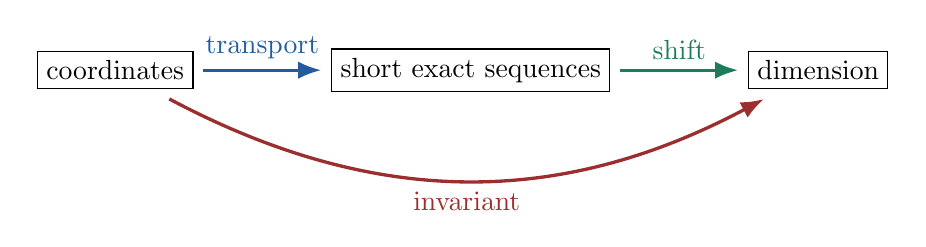
\begin{tikzpicture}[>=Latex]
\node (a) {$\boxed{\text{coordinates}}$};
\node[right=15mm of a] (b) {$\boxed{\text{short exact sequences}}$};
\node[right=15mm of b] (c) {$\boxed{\text{dimension}}$};
\draw[->,very thick,blue] (a)--node[above]{transport}(b);
\draw[->,very thick,green] (b)--node[above]{shift}(c);
\draw[->,very thick,red,bend right=28] (a) to node[below]{invariant} (c);
\end{tikzpicture}
\end{center}

\end{document}
